 \documentclass[a4paper,10pt]{article}
\input{/Users/WannaGetHigh/workspace/latex/macros.tex}

\title{TP 2 Segmentation d'une image de luminance}
\author{Fran\c cois \bsc{Lepan}}

\begin{document}
\maketitle

\section{Macro seuillage automatique des niveaux de gris par la m\'ethode de Otsu}

\begin{Verbatim}[commandchars=\\\{\}]
\codeRed{macro "OTSU" \{}

	image = getImageID();

	W = getWidth();
	H = getHeight();

	run("Duplicate...", "title=binarisee");
	image_binaire = getImageID();

	getHistogram (level,histo,256);

	max = 0;
	omega0 = 0;
	seuil = 0;

	for ( t = 1; t<= 255; t++ ) \{

		\codeBlue{histogramme cumul\'e}
		omega0 += histo[t];

		omega1 = W*H - omega0;

		\codeBlue{// centre de gravite}
		mu0 = 0;
		for ( j =0 ; j<= t; j++) \{
			mu0 += (j * histo[j]) / omega0;
		\}
		
		mu1 = 0;
		for ( k =t+1 ; k<= 255; k++) \{
			mu1 += (k * histo[k]) / omega1;
		\}

		\codeBlue{// variance inter classe}
		sigmaB = sqrt( (omega0*omega1 / H*W) * pow(mu1-mu0, 2) );

		if (max < sigmaB) \{
			max = sigmaB;
			seuil = t;
		\}
	\}

	selectImage(image_binaire);

	print ("seuil max=",seuil);

	setThreshold(0, seuil);
	run("Convert to Mask");
\codeRed{\}}

\end{Verbatim}


\section{Appliquer la macro sur l'image \emph{bi\_modal},  \emph{bi\_modal2} et \emph{avion}. Quelles conclusions pouvez-vous dresser des r\'esultats obtenus ?}

On remarque que la m\'ethode d'Otsu permet de trouver un seuil automatiquement et qui soit le meilleur pour binariser l'image. En effet si on regarde l'image \emph{bi\_modal} (\emph{c.f.} ~ Fig. \ref{bi_modal}) on voit que si on choisi un seuil on doit obtenir une image ou l'on voit clairement l'apparition d'un cercle.

\begin{figure}[ht]
\begin{center}
	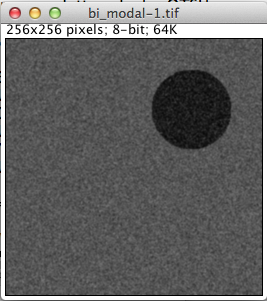
\includegraphics[width=5cm]{images/bi_modal}
\end{center}
	\caption{Image bi\_modal}
	\label{bi_modal}
\end{figure}

Apr\`es application de la m\'ethode d'Otsu on obtient la Fig.\ref{binarisee} suivante : 

\begin{figure}[ht]
\begin{center}
	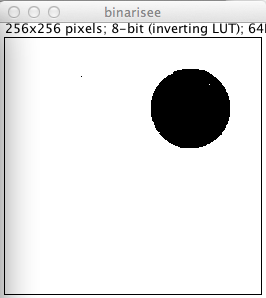
\includegraphics[width=5cm]{images/bi_modal_binarisee}
\end{center}
	\caption{Image bi\_modal binaris\'ee}
	\label{binarisee}
\end{figure}

\newpage

Voici les r\'esultat pour les deux images suivantes (\emph{bi\_modal2} et \emph{avion}) :

\begin{figure}[ht]
\begin{center}
	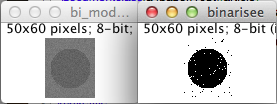
\includegraphics[width=13cm]{images/bi_modal_2}
\end{center}
	\caption{\`A gauche l'image \emph{bi\_modal2} et \`a droite la m\^eme image binaris\'ee par la m\'ethode d'Otsu}
	\label{}
\end{figure}

\begin{figure}[ht]
\begin{center}
	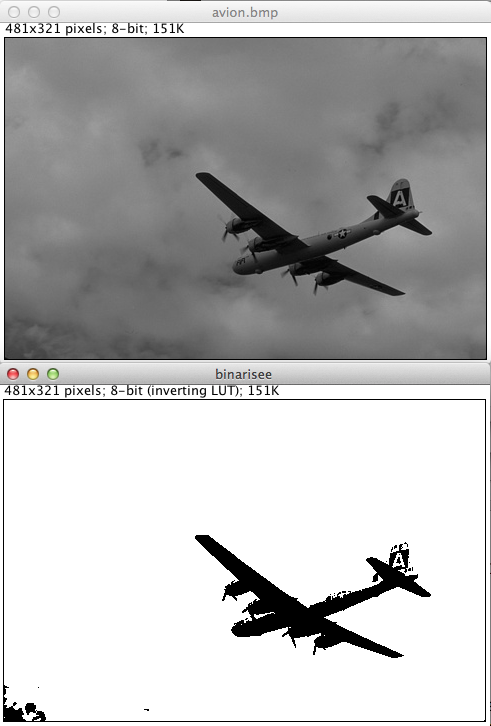
\includegraphics[width=15cm]{images/avion}
\end{center}
	\caption{Au dessus l'image \emph{avion} et en dessous la m\^eme image binaris\'ee par la m\'ethode d'Otsu}
	\label{}
\end{figure}


\end{document}